\documentclass[conference]{IEEEtran}
\IEEEoverridecommandlockouts
% The preceding line is only needed to identify funding in the first footnote. If that is unneeded, please comment it out.
\usepackage{acronym}

\usepackage{esvect}

\usepackage{listings}

\acrodef{PSO}[PSO]{\emph{particle swarm optimisation algorithm}}
\acrodef{VEPSO}[VEPSO]{\emph{vector evaluated particle swarm optimization}}
\acrodef{NN}[NN]{\emph{neural network}}
\acrodef{CPSO}[CPSO]{\emph{chaotic particle swarm optimisation algorithm}}
\acrodef{RNG}[RNG]{\emph{random number generator}}
\acrodef{CPRNG}[CPRNG]{\emph{chaotic pseudo-random number generator}}
\acrodef{VN}[VN]{\emph{Von Neumann}}
\acrodef{MSE}[MSE]{\emph{mean squared error}}
\usepackage{cite}
\usepackage{amsmath,amssymb,amsfonts}
\usepackage{commath}
\usepackage{algorithmic}
\usepackage{array,multirow,graphicx}
\usepackage{textcomp}
\def\BibTeX{{\rm B\kern-.05em{\sc i\kern-.025em b}\kern-.08em
    T\kern-.1667em\lower.7ex\hbox{E}\kern-.125emX}}
\begin{document}

\title{Multiple Sequence Alignment using Multi-Objective Particle Swarm Optimization\\
}

\author{\IEEEauthorblockN{\\Quinton Weenink}
\IEEEauthorblockA{\textit{dept. Computer Science} \\
\textit{University of Pretoria}\\
Pretoria, South Africa \\
u13176545@tuks.co.za}
}

\maketitle

\section{Introduction}
This paper aims to investigate how to achieve multiple sequence alignment using a multi-objective \ac{PSO}. While many multi-objective optimisation techniques exist this paper will investigate the performance of \ac{VEPSO} to optimise the required objectives.

\section{Background}
Sequence alignment is a way of arranging the sequences to identify regions of similarity. For this research we will be attempting to align the sequences by identifying multiple objectives and attempting to solve them, namely:
\begin{itemize}
	\item maximise the number of vertically aligned characters, while simultaneously
	\item minimising the number of leading spaces inserted.
\end{itemize}

An example of such a sequence is as follows:
\begin{lstlisting}
        a b c d e f
        b b d h g
        c a b f
\end{lstlisting}

A possible solution to the above sequence is:

\begin{lstlisting}
        - a b - c d e f - -
        - - b b - d - - h g
        c a b - - - - f - -
\end{lstlisting}

\subsection{Fitness}
\noindent The following describes how the fitness will be calculated for each of the objectives
\subsubsection{Alignment fitness}
The alignment fitness is calculated by incriminating the fitness each time the same character is aligned. Furthermore the fitness is decreased when different characters are aligned. The result is then negated in order to make both objectives minimisation problems. A solution who's characters are misaligned is considered an in-valid solution for this research.

\subsubsection{Leading space fitness}
The leading space fitness is calculated by adding the number of spaces that the solution requires.

The objective fitness for the above solution would be:
\begin{itemize}
	\item Alignment fitness $= -(1 + 2 + 1 + 1) = -5$
	\item Leading space fitness $= 15$
\end{itemize}
\subsection{Position}
Each particle will have a position that corresponds to each of the characters. For the above sequence that means a position vector of size 15 where $x_j \in [0, 7]$. Positions are floored in order to get the number of spaces to be inserted before the characters.


\section{Original Particle Swarm Optimization}
A \ac{PSO} is a machine learning algorithm where each particle moves around the search space attempting to find the optimal solution with the influence of its neighbouring particles. The position for each particle iteration is calculated as follows.

\begin{equation} \label{eq:pso:update-position}
\vec{x}_{i}^{\,t} = \vec{x}_{i}^{\,t-1} + \vec{v}_{i}^{\,t}
\end{equation}

\noindent Where:
\begin{itemize}
	\item $ \vec{x} $ is the particle position vector in n-dimensions
	\item $ \vec{v} $ is the particle velocity vector, used to calculate the particles next position
	\item $t$ is the time increment
	\item $i$ is the particle number
\end{itemize}
\vspace{5mm}
\noindent For each iteration of the algorithm, a new location of the particle is calculated based on its previous location and velocity vector as seen in (\ref{eq:pso:update-position}). The following describes a the velocity update algorithm.

\begin{equation} \label{eq:pso:update-velocity}
\vec{v}_{i}^{\,t} = w . \vec{v}_{i}^{\,t-1} + c_1 . \vec{r}_{1}^{\,t} . (\vec{x}_{pBest, i} - \vec{x}_{i}^{t-1}) + c_2 . \vec{r}_{2}^{\,t} . (\vec{x}_{nBest, i} - \vec{x}_{i}^{t-1})
\end{equation}

\noindent Where:
\begin{itemize}
	\item $c_1$ is the acceleration coefficient for the cognitive component
	\item $c_2$ is the acceleration coefficient for the social component
	\item $r_1$ and $r_2$ is a vector of random numbers in the range (0, 1)
	\item $\vec{x}_{pBest}$ is the personal best position of that particle
	\item $\vec{x}_{nBest}$ is the best position found in that particles neighbourhood
\end{itemize}
\vspace{5mm}
\noindent Particle's social component, the third term in (\ref{eq:pso:update-velocity}), requires $ nBest $, the best neighbouring particles position. The set of neighbouring particles is determined by the topology used in the \ac{PSO}. Different topologies could influence the performance of the \ac{PSO}.

    \subsection{Social Network Topologies}
    
    In the above mentioned \ac{PSO} the neighbourhood could be described in a variety of ways. One such method is the $ gBest $ topology, where each particle is a neighbour of every other particle in the network. This means that the particle's $ nBest $ is always the global best particle for the swarm. 
    
    Another social topology called $ lBest $ connects particles in a ring topology, the neighbourhood is specified by a fixed size of $ n_s $. The $ nBest $ in this case is determined by the best particle within $ n_s $ neighbours from the current particle\cite{vanwyk:overfitting-psoffnn}. 
    
\section{Vector Evaluated Particle Swarm Optimization}
In this multi-swarm concept, each objective function is optimised by a swarm of particles using the $gBest$ from another swarm\cite{kian-lim:pso}.

While position for each particle is updated in the same way as an original \ac{PSO} the velocity update function changes. Assuming a multi-objective problem with 2 objectives the following describes the velocity update for each of the swarms.

\begin{equation} \label{eq:vepso:update-velocity}
\begin{array}{l}
S_1.\vec{v}_{i}^{\,t} = w . S_1 . \vec{v}_{i}^{\,t-1} + c_1 . \vec{r}_{1}^{\,t} . (S_1 . \vec{x}_{pBest, i} - S_1 . \vec{x}_{i}^{t-1})\\
\hspace{29mm} + c_2 . \vec{r}_{2}^{\,t} . (S_2 . \vec{x}_{nBest, i} - S_1 . \vec{x}_{i}^{t-1})
\end{array}
\end{equation}

\begin{equation} \label{eq:vepso:update-velocity2}
\begin{array}{l}
S_2.\vec{v}_{i}^{\,t} = w . S_2 . \vec{v}_{i}^{\,t-1} + c_1 . \vec{r}_{1}^{\,t} . (S_2 . \vec{x}_{pBest, i} - S_2 . \vec{x}_{i}^{t-1})\\
\hspace{29mm} + c_2 . \vec{r}_{2}^{\,t} . (S_1 . \vec{x}_{nBest, i} - S_2 . \vec{x}_{i}^{t-1})
\end{array}
\end{equation}

\noindent Where:
\begin{itemize}
    \item $S_1$ and $S_2$ are the values associated with swarm 1 and swarm 2 respectively
	\item There rest remain the same as in the original pso velocity update function (\ref{eq:pso:update-velocity})
\end{itemize}
\vspace{5mm}

\subsection{Swarm Social Network Topologies}

Similarly to the social network topologies mentioned in for the original \ac{PSO} the same topologies apply to \ac{VEPSO}. In the same way the $lBest$ functions for particle social topologies the swarm discussed will share information to the next swarm in the same way.

$pBest$ and $nBest$ positions were only used as a local or global guide if they were non-dominated by a previous solution as well as a valid solution.

\subsection{Objectives}

Each of the swarm's error functions is the resulting fitness of one of the objectives. A good multi-objective optimisation algorithm should be able to solve its own objective while not forgetting about the other swarms objectives.

\subsection{Boundary Constraint Handling Mechanisms}

The the boundary constraint clamping approach used in this research to prevent particles from leaving the search space. If a particle violates a boundary constraint in a specific dimension, then the particles position was clamped to the edge of the constraint. For this research this was specified by the max length of the sequences.

\section{Experiments}
    \subsection{\ac{PSO} configuration}
    In order to achieve viable results, each experiment was run as a mean over 30 samples. $r_1$ and $r_2$ sampled from a uniform distribution $ (0, 1) $ as specified in equation \ref{eq:pso:update-velocity}.
    
    A memory based \ac{PSO} was used with a star or $ gBest $ social topologie. 
    
    50 particles were used for all functions. 
    
    The constants $ c_1 = c_2 = 1.4 $ as well $ w = 0.7 $ were set as suggested in \cite{vanwyk:overfitting-psoffnn}. 
    
    No $ V_{max} $ was used during this study.

\section{Results}


\begin{table}[htbp]
\caption{Results after 2000 iterations. Means are reported over 30 samples with standard deviations in parenthesis}
\begin{center}
\begin{tabular}{|c|c|c|c|c|}
\hline
& & $ f_1 $ & $ f_2 $ & $ f_3 $\\\hline
\multirow{4}{*}{$ S_1 $} &
\multirow{2}{*}{$ f1 $} &
-4.2666666 & -5.6333333 & -3.93333333\\
&&(0.7272474) & (1.0159833) & (0.2494438)\\
&\multirow{2}{*}{$ f2 $} &
40.6 & 86.5 & 45.7\\
&&(11.842297) & (14.6986393) & (10.030453)\\
\hline
\multirow{4}{*}{$ S_2 $} &
\multirow{2}{*}{$ f1 $} &
-0.866666 & -2.6333333 & -2.1\\
&&(4.74505590) & (3.69218393) & (3.02599845)\\
&\multirow{2}{*}{$ f2 $} &
27.2 & 73.3 & 30.1\\
&&(5.3628350) & (7.6164296) & (4.7423622)\\
\hline
\end{tabular}
\label{tab:glass}
\end{center}
\end{table}

Figures (\ref{fig:f1:fitness}, \ref{fig:f2:fitness}, \ref{fig:f3:fitness}) indicated the objective's fitness over the 2000 iterations that these solutions were trained over. It can be observed that each swarm is attempting to achieve result best for their objective. Each swarm being the best fitness for its particular objective.

One can also observe the objectives of each swarm approaching each other as their results are influenced by the global guides that are effecting their velocity.

\begin{figure}[htbp]
\centerline{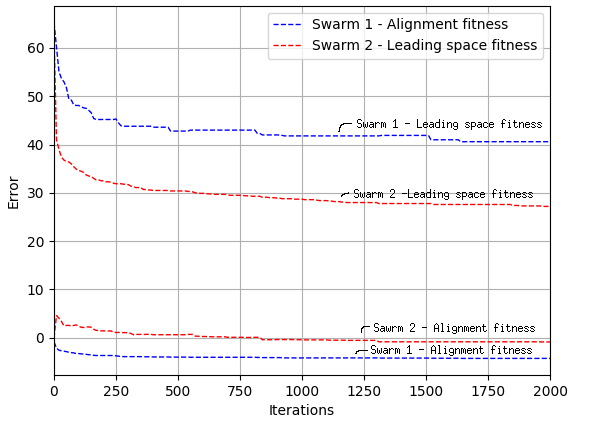
\includegraphics[width=90mm]{images/results/f1-fitness.png}}
\caption{$f_1$'s fitness objectives over time }
\label{fig:f1:fitness}
\end{figure}

\begin{figure}[htbp]
\centerline{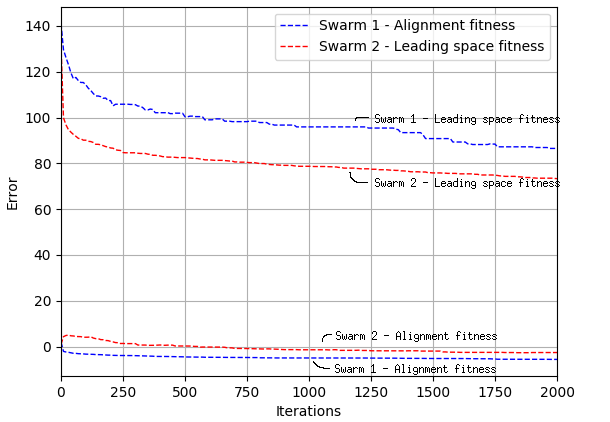
\includegraphics[width=90mm]{images/results/f2-fitness.png}}
\caption{$f_2$'s fitness objectives over time }
\label{fig:f2:fitness}
\end{figure}

\begin{figure}[htbp]
\centerline{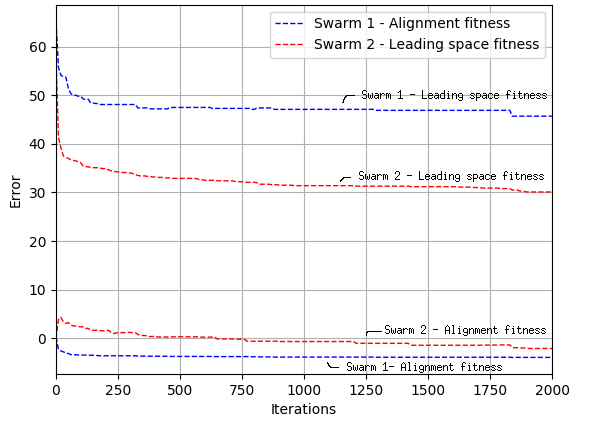
\includegraphics[width=90mm]{images/results/f3-fitness.png}}
\caption{$f_3$'s fitness objectives over time }
\label{fig:f3:fitness}
\end{figure}


\newpage
Figures (\ref{fig:f1:solutions}, \ref{fig:f2:solutions}, \ref{fig:f3:solutions}) plot the solutions according to their swarm (x-axis: Alignment fitness, y-axis: Leading space fitness). For each of the testing sequences one can see that the swarms form what appears to be a Pareto front \cite{kian-lim:pso}. This being the place where the one objective can't improve more without negatively impacting the other. 

\begin{figure}[htbp]
\centerline{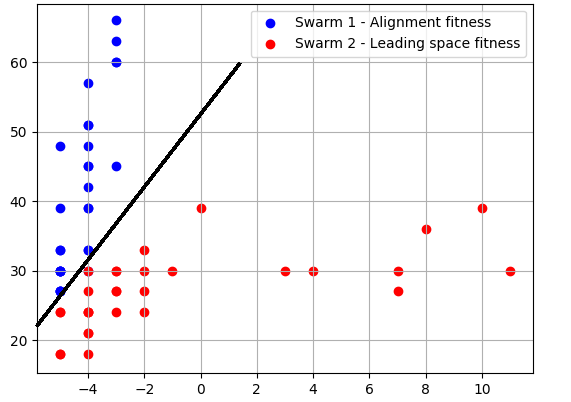
\includegraphics[width=90mm]{images/results/f1-solutions.png}}
\caption{$f_1$'s non-dominated solutions }
\label{fig:f1:solutions}
\end{figure}

\begin{figure}[htbp]
\centerline{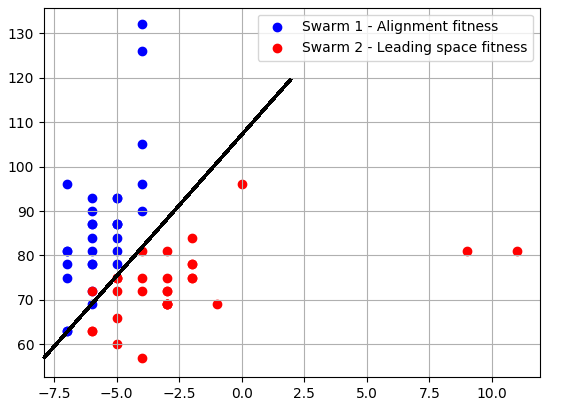
\includegraphics[width=90mm]{images/results/f2-solutions.png}}
\caption{$f_2$'s non-dominated solutions }
\label{fig:f2:solutions}
\end{figure}

\begin{figure}[htbp]
\centerline{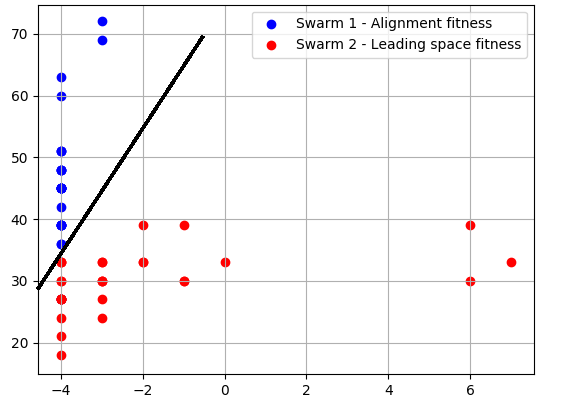
\includegraphics[width=90mm]{images/results/f3-solutions.png}}
\caption{$f_3$'s non-dominated solutions }
\label{fig:f3:solutions}
\end{figure}

\newpage
\section{Conclusion}
In conclusion one can observe the ability of \ac{VEPSO}'s in solving multiple sequence alignment problems. \ac{VEPSO} did however struggle with lager sequences like in $f_2$ and one can assume this is due to lack of exploration. The addition of achieve, as discussed in \cite{kian-lim:pso}, would significantly benefit the optimisation as well as allow the addition of multiple solutions resulting in in increased exploration.

\newpage

\nocite{*}
\noindent
\bibliographystyle{IEEEtran}
\indent
\bibliography{IEEEabrv,sbc-template}

\section{Appendix}

$f_1$, sequence provided, where $x_j \in [0, 7]$
\begin{lstlisting}
        a b c d e f
        b b d h g
        c a b f
\end{lstlisting}

$f_2$, longer sequence, where $x_j \in [0, 10]$
\begin{lstlisting}
        a b c d e f a a h
        f b b d h g h h
        c a b f f e a
\end{lstlisting}

$f_3$, a sequence that would benefit from bounds bigger than the number of sequences, where $x_j \in [0, 7]$
\begin{lstlisting}
        a b c d e f
        g h i j k
        a b c d
\end{lstlisting}

\end{document}
